\documentclass[1p]{elsarticle_modified}
%\bibliographystyle{elsarticle-num}

%\usepackage[colorlinks]{hyperref}
%\usepackage{abbrmath_seonhwa} %\Abb, \Ascr, \Acal ,\Abf, \Afrak
\usepackage{amsfonts}
\usepackage{amssymb}
\usepackage{amsmath}
\usepackage{amsthm}
\usepackage{scalefnt}
\usepackage{amsbsy}
\usepackage{kotex}
\usepackage{caption}
\usepackage{subfig}
\usepackage{color}
\usepackage{graphicx}
\usepackage{xcolor} %% white, black, red, green, blue, cyan, magenta, yellow
\usepackage{float}
\usepackage{setspace}
\usepackage{hyperref}

\usepackage{tikz}
\usetikzlibrary{arrows}

\usepackage{multirow}
\usepackage{array} % fixed length table
\usepackage{hhline}

%%%%%%%%%%%%%%%%%%%%%
\makeatletter
\renewcommand*\env@matrix[1][\arraystretch]{%
	\edef\arraystretch{#1}%
	\hskip -\arraycolsep
	\let\@ifnextchar\new@ifnextchar
	\array{*\c@MaxMatrixCols c}}
\makeatother %https://tex.stackexchange.com/questions/14071/how-can-i-increase-the-line-spacing-in-a-matrix
%%%%%%%%%%%%%%%

\usepackage[normalem]{ulem}

\newcommand{\msout}[1]{\ifmmode\text{\sout{\ensuremath{#1}}}\else\sout{#1}\fi}
%SOURCE: \msout is \stkout macro in https://tex.stackexchange.com/questions/20609/strikeout-in-math-mode

\newcommand{\cancel}[1]{
	\ifmmode
	{\color{red}\msout{#1}}
	\else
	{\color{red}\sout{#1}}
	\fi
}

\newcommand{\add}[1]{
	{\color{blue}\uwave{#1}}
}

\newcommand{\replace}[2]{
	\ifmmode
	{\color{red}\msout{#1}}{\color{blue}\uwave{#2}}
	\else
	{\color{red}\sout{#1}}{\color{blue}\uwave{#2}}
	\fi
}

\newcommand{\Sol}{\mathcal{S}} %segment
\newcommand{\D}{D} %diagram
\newcommand{\A}{\mathcal{A}} %arc


%%%%%%%%%%%%%%%%%%%%%%%%%%%%%5 test

\def\sl{\operatorname{\textup{SL}}(2,\Cbb)}
\def\psl{\operatorname{\textup{PSL}}(2,\Cbb)}
\def\quan{\mkern 1mu \triangleright \mkern 1mu}

\theoremstyle{definition}
\newtheorem{thm}{Theorem}[section]
\newtheorem{prop}[thm]{Proposition}
\newtheorem{lem}[thm]{Lemma}
\newtheorem{ques}[thm]{Question}
\newtheorem{cor}[thm]{Corollary}
\newtheorem{defn}[thm]{Definition}
\newtheorem{exam}[thm]{Example}
\newtheorem{rmk}[thm]{Remark}
\newtheorem{alg}[thm]{Algorithm}

\newcommand{\I}{\sqrt{-1}}
\begin{document}

%\begin{frontmatter}
%
%\title{Boundary parabolic representations of knots up to 8 crossings}
%
%%% Group authors per affiliation:
%\author{Yunhi Cho} 
%\address{Department of Mathematics, University of Seoul, Seoul, Korea}
%\ead{yhcho@uos.ac.kr}
%
%
%\author{Seonhwa Kim} %\fnref{s_kim}}
%\address{Center for Geometry and Physics, Institute for Basic Science, Pohang, 37673, Korea}
%\ead{ryeona17@ibs.re.kr}
%
%\author{Hyuk Kim}
%\address{Department of Mathematical Sciences, Seoul National University, Seoul 08826, Korea}
%\ead{hyukkim@snu.ac.kr}
%
%\author{Seokbeom Yoon}
%\address{Department of Mathematical Sciences, Seoul National University, Seoul, 08826,  Korea}
%\ead{sbyoon15@snu.ac.kr}
%
%\begin{abstract}
%We find all boundary parabolic representation of knots up to 8 crossings.
%
%\end{abstract}
%\begin{keyword}
%    \MSC[2010] 57M25 
%\end{keyword}
%
%\end{frontmatter}

%\linenumbers
%\tableofcontents
%
\newcommand\colored[1]{\textcolor{white}{\rule[-0.35ex]{0.8em}{1.4ex}}\kern-0.8em\color{red} #1}%
%\newcommand\colored[1]{\textcolor{white}{ #1}\kern-2.17ex	\textcolor{white}{ #1}\kern-1.81ex	\textcolor{white}{ #1}\kern-2.15ex\color{red}#1	}

{\Large $\underline{12n_{0706}~(K12n_{0706})}$}

\setlength{\tabcolsep}{10pt}
\renewcommand{\arraystretch}{1.6}
\vspace{1cm}\begin{tabular}{m{100pt}>{\centering\arraybackslash}m{274pt}}
\multirow{5}{120pt}{
	\centering
	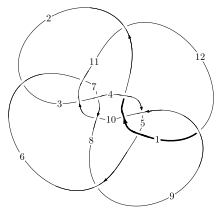
\includegraphics[width=112pt]{../../../GIT/diagram.site/Diagrams/png/2795_12n_0706.png}\\
\ \ \ A knot diagram\footnotemark}&
\allowdisplaybreaks
\textbf{Linearized knot diagam} \\
\cline{2-2}
 &
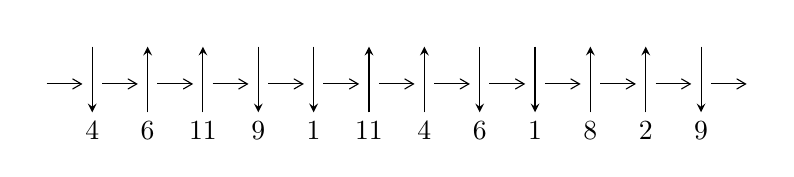
\begin{tikzpicture}[x=20pt, y=17pt]
	% nodes
	\node (C0) at (0, 0) {};
	\node (C1) at (1, 0) {};
	\node (C1U) at (1, +1) {};
	\node (C1D) at (1, -1) {4};

	\node (C2) at (2, 0) {};
	\node (C2U) at (2, +1) {};
	\node (C2D) at (2, -1) {6};

	\node (C3) at (3, 0) {};
	\node (C3U) at (3, +1) {};
	\node (C3D) at (3, -1) {11};

	\node (C4) at (4, 0) {};
	\node (C4U) at (4, +1) {};
	\node (C4D) at (4, -1) {9};

	\node (C5) at (5, 0) {};
	\node (C5U) at (5, +1) {};
	\node (C5D) at (5, -1) {1};

	\node (C6) at (6, 0) {};
	\node (C6U) at (6, +1) {};
	\node (C6D) at (6, -1) {11};

	\node (C7) at (7, 0) {};
	\node (C7U) at (7, +1) {};
	\node (C7D) at (7, -1) {4};

	\node (C8) at (8, 0) {};
	\node (C8U) at (8, +1) {};
	\node (C8D) at (8, -1) {6};

	\node (C9) at (9, 0) {};
	\node (C9U) at (9, +1) {};
	\node (C9D) at (9, -1) {1};

	\node (C10) at (10, 0) {};
	\node (C10U) at (10, +1) {};
	\node (C10D) at (10, -1) {8};

	\node (C11) at (11, 0) {};
	\node (C11U) at (11, +1) {};
	\node (C11D) at (11, -1) {2};

	\node (C12) at (12, 0) {};
	\node (C12U) at (12, +1) {};
	\node (C12D) at (12, -1) {9};
	\node (C13) at (13, 0) {};

	% arrows
	\draw[->,>={angle 60}]
	(C0) edge (C1) (C1) edge (C2) (C2) edge (C3) (C3) edge (C4) (C4) edge (C5) (C5) edge (C6) (C6) edge (C7) (C7) edge (C8) (C8) edge (C9) (C9) edge (C10) (C10) edge (C11) (C11) edge (C12) (C12) edge (C13) ;	\draw[->,>=stealth]
	(C1U) edge (C1D) (C2D) edge (C2U) (C3D) edge (C3U) (C4U) edge (C4D) (C5U) edge (C5D) (C6D) edge (C6U) (C7D) edge (C7U) (C8U) edge (C8D) (C9U) edge (C9D) (C10D) edge (C10U) (C11D) edge (C11U) (C12U) edge (C12D) ;
	\end{tikzpicture} \\
\hhline{~~} \\& 
\textbf{Solving Sequence} \\ \cline{2-2} 
 &
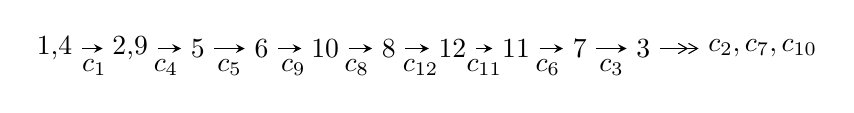
\begin{tikzpicture}[x=23pt, y=7pt]
	% node
	\node (A0) at (-1/8, 0) {1,4};
	\node (A1) at (17/16, 0) {2,9};
	\node (A2) at (17/8, 0) {5};
	\node (A3) at (25/8, 0) {6};
	\node (A4) at (33/8, 0) {10};
	\node (A5) at (41/8, 0) {8};
	\node (A6) at (49/8, 0) {12};
	\node (A7) at (57/8, 0) {11};
	\node (A8) at (65/8, 0) {7};
	\node (A9) at (73/8, 0) {3};
	\node (C1) at (1/2, -1) {$c_{1}$};
	\node (C2) at (13/8, -1) {$c_{4}$};
	\node (C3) at (21/8, -1) {$c_{5}$};
	\node (C4) at (29/8, -1) {$c_{9}$};
	\node (C5) at (37/8, -1) {$c_{8}$};
	\node (C6) at (45/8, -1) {$c_{12}$};
	\node (C7) at (53/8, -1) {$c_{11}$};
	\node (C8) at (61/8, -1) {$c_{6}$};
	\node (C9) at (69/8, -1) {$c_{3}$};
	\node (A10) at (11, 0) {$c_{2},c_{7},c_{10}$};

	% edge
	\draw[->,>=stealth]	
	(A0) edge (A1) (A1) edge (A2) (A2) edge (A3) (A3) edge (A4) (A4) edge (A5) (A5) edge (A6) (A6) edge (A7) (A7) edge (A8) (A8) edge (A9) ;
	\draw[->>,>={angle 60}]	
	(A9) edge (A10);
\end{tikzpicture} \\ 

\end{tabular} \\

\footnotetext{
The image of knot diagram is generated by the software ``\textbf{Draw programme}" developed by Andrew Bartholomew(\url{http://www.layer8.co.uk/maths/draw/index.htm\#Running-draw}), where we modified some parts for our purpose(\url{https://github.com/CATsTAILs/LinksPainter}).
}\phantom \\ \newline 
\centering \textbf{Ideals for irreducible components\footnotemark of $X_{\text{par}}$} 
 
\begin{align*}
I^u_{1}&=\langle 
u^3+2 u^2+2 b+u,\;- u^2+2 a-2 u-1,\;u^4+2 u^3+2 u^2-2 u+1\rangle \\
I^u_{2}&=\langle 
u^5- u^4-2 u^2+4 b+3 u-1,\;u^5+u^4-2 u^3+12 a-3 u+7,\;u^6-2 u^5+u^4+3 u^2-2 u+3\rangle \\
I^u_{3}&=\langle 
u^5-2 u^4- u^3+5 u^2+2 b+3 u-4,\;-2 u^5+2 u^4+3 u^3-7 u^2+6 a-6 u+3,\;u^6-2 u^5- u^4+6 u^3-6 u+3\rangle \\
I^u_{4}&=\langle 
2 u^5- u^4-5 u^3+6 u^2+6 b+9 u-6,\;-4 u^5+5 u^4+10 u^3-21 u^2+6 a-15 u+15,\\
\phantom{I^u_{4}}&\phantom{= \langle  }u^6-2 u^5- u^4+6 u^3-6 u+3\rangle \\
I^u_{5}&=\langle 
-99 u^5-258 u^4-363 u^3-295 u^2+82 b-59 u-72,\\
\phantom{I^u_{5}}&\phantom{= \langle  }-81 u^5-144 u^4-174 u^3-96 u^2+82 a-11 u-85,\;9 u^6+27 u^5+48 u^4+51 u^3+34 u^2+16 u+8\rangle \\
I^u_{6}&=\langle 
b- a,\;a^2+a-1,\;u+1\rangle \\
I^u_{7}&=\langle 
- a^2 u^2+a u+b- a- u+1,\;u^3 a^2+a u+u^2- u+1\rangle \\
\\
\end{align*}
\raggedright * 6 irreducible components of $\dim_{\mathbb{C}}=0$, with total 30 representations.\\
\raggedright * 1 irreducible components of $\dim_{\mathbb{C}}=1$ \\
\footnotetext{All coefficients of polynomials are rational numbers. But the coefficients are sometimes approximated in decimal forms when there is not enough margin.}
\newpage
\renewcommand{\arraystretch}{1}
\centering \section*{I. $I^u_{1}= \langle u^3+2 u^2+2 b+u,\;- u^2+2 a-2 u-1,\;u^4+2 u^3+2 u^2-2 u+1 \rangle$}
\flushleft \textbf{(i) Arc colorings}\\
\begin{tabular}{m{7pt} m{180pt} m{7pt} m{180pt} }
\flushright $a_{1}=$&$\begin{pmatrix}1\\0\end{pmatrix}$ \\
\flushright $a_{4}=$&$\begin{pmatrix}0\\u\end{pmatrix}$ \\
\flushright $a_{2}=$&$\begin{pmatrix}1\\u^2\end{pmatrix}$ \\
\flushright $a_{9}=$&$\begin{pmatrix}\frac{1}{2} u^2+u+\frac{1}{2}\\-\frac{1}{2} u^3- u^2-\frac{1}{2} u\end{pmatrix}$ \\
\flushright $a_{5}=$&$\begin{pmatrix}-\frac{1}{2} u^2- u+\frac{1}{2}\\\frac{1}{2} u^3+u^2+\frac{1}{2} u\end{pmatrix}$ \\
\flushright $a_{6}=$&$\begin{pmatrix}-\frac{1}{2} u^3-\frac{3}{2} u^2-\frac{3}{2} u+\frac{1}{2}\\\frac{1}{2} u^3+u^2+\frac{1}{2} u\end{pmatrix}$ \\
\flushright $a_{10}=$&$\begin{pmatrix}\frac{1}{2} u^3+\frac{3}{2} u^2+\frac{3}{2} u+\frac{1}{2}\\-\frac{1}{2} u^3- u^2-\frac{1}{2} u\end{pmatrix}$ \\
\flushright $a_{8}=$&$\begin{pmatrix}\frac{1}{2} u^3+u^2+\frac{3}{2} u\\-\frac{1}{2} u^3-\frac{1}{2} u^2-\frac{3}{2} u+\frac{1}{2}\end{pmatrix}$ \\
\flushright $a_{12}=$&$\begin{pmatrix}\frac{1}{2} u^2+u+\frac{1}{2}\\-\frac{1}{2} u^3- u^2+\frac{1}{2} u\end{pmatrix}$ \\
\flushright $a_{11}=$&$\begin{pmatrix}\frac{1}{2} u^3+u^2+\frac{3}{2} u\\\frac{1}{2} u^2- u+\frac{1}{2}\end{pmatrix}$ \\
\flushright $a_{7}=$&$\begin{pmatrix}-\frac{1}{2} u^3- u^2-\frac{3}{2} u\\-\frac{1}{2} u^2+2 u-\frac{1}{2}\end{pmatrix}$ \\
\flushright $a_{3}=$&$\begin{pmatrix}-\frac{1}{2} u^2+\frac{1}{2}\\\frac{1}{2} u^3+\frac{3}{2} u^2-\frac{1}{2} u+\frac{1}{2}\end{pmatrix}$\\&\end{tabular}
\flushleft \textbf{(ii) Obstruction class $= -1$}\\~\\
\flushleft \textbf{(iii) Cusp Shapes $= 3 u^3+9 u^2+9 u-3$}\\~\\
\newpage\renewcommand{\arraystretch}{1}
\flushleft \textbf{(iv) u-Polynomials at the component}\newline \\
\begin{tabular}{m{50pt}|m{274pt}}
Crossings & \hspace{64pt}u-Polynomials at each crossing \\
\hline $$\begin{aligned}c_{1},c_{8}\end{aligned}$$&$\begin{aligned}
&u^4-2 u^3+2 u^2+2 u+1
\end{aligned}$\\
\hline $$\begin{aligned}c_{2},c_{3},c_{6}\\c_{7}\end{aligned}$$&$\begin{aligned}
&u^4-4 u^3+5 u^2-2 u+1
\end{aligned}$\\
\hline $$\begin{aligned}c_{4},c_{5},c_{9}\\c_{12}\end{aligned}$$&$\begin{aligned}
&u^4+4 u^3+5 u^2+2 u+1
\end{aligned}$\\
\hline $$\begin{aligned}c_{10},c_{11}\end{aligned}$$&$\begin{aligned}
&u^4+2 u^3+2 u^2-2 u+1
\end{aligned}$\\
\hline
\end{tabular}\\~\\
\newpage\renewcommand{\arraystretch}{1}
\flushleft \textbf{(v) Riley Polynomials at the component}\newline \\
\begin{tabular}{m{50pt}|m{274pt}}
Crossings & \hspace{64pt}Riley Polynomials at each crossing \\
\hline $$\begin{aligned}c_{1},c_{8},c_{10}\\c_{11}\end{aligned}$$&$\begin{aligned}
&y^4+14 y^2+1
\end{aligned}$\\
\hline $$\begin{aligned}c_{2},c_{3},c_{4}\\c_{5},c_{6},c_{7}\\c_{9},c_{12}\end{aligned}$$&$\begin{aligned}
&y^4-6 y^3+11 y^2+6 y+1
\end{aligned}$\\
\hline
\end{tabular}\\~\\
\newpage\flushleft \textbf{(vi) Complex Volumes and Cusp Shapes}
$$\begin{array}{c|c|c}  
\text{Solutions to }I^u_{1}& \I (\text{vol} + \sqrt{-1}CS) & \text{Cusp shape}\\
 \hline 
\begin{aligned}
u &= \phantom{-}0.366025 + 0.366025 I \\
a &= \phantom{-}0.866025 + 0.500000 I \\
b &= -0.133975 - 0.500000 I\end{aligned}
 & \phantom{-0.000000 } -1.23808 I & \phantom{-0.000000 -}0. + 6.00000 I \\ \hline\begin{aligned}
u &= \phantom{-}0.366025 - 0.366025 I \\
a &= \phantom{-}0.866025 - 0.500000 I \\
b &= -0.133975 + 0.500000 I\end{aligned}
 & \phantom{-0.000000 -}1.23808 I & \phantom{-0.000000 } 0. - 6.00000 I \\ \hline\begin{aligned}
u &= -1.36603 + 1.36603 I \\
a &= -0.866025 - 0.500000 I \\
b &= -1.86603 + 0.50000 I\end{aligned}
 & \phantom{-0.000000 -}13.4174 I & \phantom{-0.000000 } 0. - 6.00000 I \\ \hline\begin{aligned}
u &= -1.36603 - 1.36603 I \\
a &= -0.866025 + 0.500000 I \\
b &= -1.86603 - 0.50000 I\end{aligned}
 & \phantom{-0.000000 } -13.4174 I & \phantom{-0.000000 -}0. + 6.00000 I\\
 \hline 
 \end{array}$$\newpage\newpage\renewcommand{\arraystretch}{1}
\centering \section*{II. $I^u_{2}= \langle u^5- u^4-2 u^2+4 b+3 u-1,\;u^5+u^4-2 u^3+12 a-3 u+7,\;u^6-2 u^5+u^4+3 u^2-2 u+3 \rangle$}
\flushleft \textbf{(i) Arc colorings}\\
\begin{tabular}{m{7pt} m{180pt} m{7pt} m{180pt} }
\flushright $a_{1}=$&$\begin{pmatrix}1\\0\end{pmatrix}$ \\
\flushright $a_{4}=$&$\begin{pmatrix}0\\u\end{pmatrix}$ \\
\flushright $a_{2}=$&$\begin{pmatrix}1\\u^2\end{pmatrix}$ \\
\flushright $a_{9}=$&$\begin{pmatrix}-\frac{1}{12} u^5-\frac{1}{12} u^4+\cdots+\frac{1}{4} u-\frac{7}{12}\\-\frac{1}{4} u^5+\frac{1}{4} u^4+\cdots-\frac{3}{4} u+\frac{1}{4}\end{pmatrix}$ \\
\flushright $a_{5}=$&$\begin{pmatrix}\frac{1}{12} u^5+\frac{1}{12} u^4+\cdots-\frac{1}{4} u-\frac{5}{12}\\\frac{1}{4} u^5-\frac{1}{4} u^4+\cdots+\frac{3}{4} u-\frac{1}{4}\end{pmatrix}$ \\
\flushright $a_{6}=$&$\begin{pmatrix}-\frac{1}{6} u^5+\frac{1}{3} u^4+\cdots- u-\frac{1}{6}\\\frac{1}{4} u^5-\frac{1}{4} u^4+\cdots+\frac{3}{4} u-\frac{1}{4}\end{pmatrix}$ \\
\flushright $a_{10}=$&$\begin{pmatrix}\frac{1}{6} u^5-\frac{1}{3} u^4+\cdots+u-\frac{5}{6}\\-\frac{1}{4} u^5+\frac{1}{4} u^4+\cdots-\frac{3}{4} u+\frac{1}{4}\end{pmatrix}$ \\
\flushright $a_{8}=$&$\begin{pmatrix}-\frac{1}{12} u^5-\frac{1}{12} u^4+\cdots-\frac{1}{4} u-\frac{1}{12}\\-\frac{1}{2} u^3+\frac{1}{2} u^2-\frac{1}{2} u-\frac{1}{2}\end{pmatrix}$ \\
\flushright $a_{12}=$&$\begin{pmatrix}\frac{1}{12} u^5+\frac{1}{12} u^4+\cdots-\frac{1}{4} u+\frac{7}{12}\\\frac{1}{4} u^5-\frac{1}{4} u^4+\cdots-\frac{1}{4} u-\frac{1}{4}\end{pmatrix}$ \\
\flushright $a_{11}=$&$\begin{pmatrix}\frac{1}{12} u^5+\frac{1}{12} u^4+\cdots+\frac{1}{4} u+\frac{1}{12}\\-\frac{1}{4} u^5+\frac{1}{4} u^4+\cdots-\frac{1}{4} u-\frac{1}{4}\end{pmatrix}$ \\
\flushright $a_{7}=$&$\begin{pmatrix}-\frac{1}{12} u^5-\frac{1}{12} u^4+\cdots-\frac{1}{4} u-\frac{1}{12}\\\frac{1}{4} u^5-\frac{1}{4} u^4+\cdots-\frac{3}{4} u+\frac{1}{4}\end{pmatrix}$ \\
\flushright $a_{3}=$&$\begin{pmatrix}\frac{1}{12} u^5-\frac{5}{12} u^4+\cdots+\frac{3}{4} u+\frac{1}{12}\\-\frac{1}{2} u^3+\frac{3}{2} u^2-\frac{1}{2} u+\frac{1}{2}\end{pmatrix}$\\&\end{tabular}
\flushleft \textbf{(ii) Obstruction class $= 1$}\\~\\
\flushleft \textbf{(iii) Cusp Shapes $= 3 u^5-\frac{9}{2} u^4+3 u^2+6 u-\frac{3}{2}$}\\~\\
\newpage\renewcommand{\arraystretch}{1}
\flushleft \textbf{(iv) u-Polynomials at the component}\newline \\
\begin{tabular}{m{50pt}|m{274pt}}
Crossings & \hspace{64pt}u-Polynomials at each crossing \\
\hline $$\begin{aligned}c_{1},c_{10}\end{aligned}$$&$\begin{aligned}
&u^6-2 u^5+u^4+3 u^2-2 u+3
\end{aligned}$\\
\hline $$\begin{aligned}c_{2},c_{5},c_{6}\\c_{12}\end{aligned}$$&$\begin{aligned}
&u^6-3 u^5+2 u^4- u^3+2 u^2+u+1
\end{aligned}$\\
\hline $$\begin{aligned}c_{3},c_{4},c_{7}\\c_{9}\end{aligned}$$&$\begin{aligned}
&u^6+3 u^5+2 u^4+u^3+2 u^2- u+1
\end{aligned}$\\
\hline $$\begin{aligned}c_{8},c_{11}\end{aligned}$$&$\begin{aligned}
&u^6+2 u^5+u^4+3 u^2+2 u+3
\end{aligned}$\\
\hline
\end{tabular}\\~\\
\newpage\renewcommand{\arraystretch}{1}
\flushleft \textbf{(v) Riley Polynomials at the component}\newline \\
\begin{tabular}{m{50pt}|m{274pt}}
Crossings & \hspace{64pt}Riley Polynomials at each crossing \\
\hline $$\begin{aligned}c_{1},c_{8},c_{10}\\c_{11}\end{aligned}$$&$\begin{aligned}
&y^6-2 y^5+7 y^4+4 y^3+15 y^2+14 y+9
\end{aligned}$\\
\hline $$\begin{aligned}c_{2},c_{3},c_{4}\\c_{5},c_{6},c_{7}\\c_{9},c_{12}\end{aligned}$$&$\begin{aligned}
&y^6-5 y^5+2 y^4+15 y^3+10 y^2+3 y+1
\end{aligned}$\\
\hline
\end{tabular}\\~\\
\newpage\flushleft \textbf{(vi) Complex Volumes and Cusp Shapes}
$$\begin{array}{c|c|c}  
\text{Solutions to }I^u_{2}& \I (\text{vol} + \sqrt{-1}CS) & \text{Cusp shape}\\
 \hline 
\begin{aligned}
u &= \phantom{-}0.319448 + 0.816851 I \\
a &= -0.649948 + 0.216712 I \\
b &= -0.384646 - 0.461682 I\end{aligned}
 & \phantom{-0.000000 } -3.01792 I & \phantom{-0.000000 -}0. + 8.67149 I \\ \hline\begin{aligned}
u &= \phantom{-}0.319448 - 0.816851 I \\
a &= -0.649948 - 0.216712 I \\
b &= -0.384646 + 0.461682 I\end{aligned}
 & \phantom{-0.000000 -}3.01792 I & \phantom{-0.000000 } 0. - 8.67149 I \\ \hline\begin{aligned}
u &= -0.814644 + 0.831311 I \\
a &= -0.562136 + 0.513813 I \\
b &= \phantom{-}0.030802 - 0.885884 I\end{aligned}
 & \phantom{-}9.18468 + 5.87764 I & \phantom{-}6.07806 - 4.16480 I \\ \hline\begin{aligned}
u &= -0.814644 - 0.831311 I \\
a &= -0.562136 - 0.513813 I \\
b &= \phantom{-}0.030802 + 0.885884 I\end{aligned}
 & \phantom{-}9.18468 - 5.87764 I & \phantom{-}6.07806 + 4.16480 I \\ \hline\begin{aligned}
u &= \phantom{-}1.49520 + 0.80186 I \\
a &= \phantom{-}1.045420 - 0.362585 I \\
b &= \phantom{-}1.85384 + 0.29614 I\end{aligned}
 & -9.18468 - 5.87764 I & -6.07806 + 4.16480 I \\ \hline\begin{aligned}
u &= \phantom{-}1.49520 - 0.80186 I \\
a &= \phantom{-}1.045420 + 0.362585 I \\
b &= \phantom{-}1.85384 - 0.29614 I\end{aligned}
 & -9.18468 + 5.87764 I & -6.07806 - 4.16480 I\\
 \hline 
 \end{array}$$\newpage\newpage\renewcommand{\arraystretch}{1}
\centering \section*{III. $I^u_{3}= \langle u^5-2 u^4- u^3+5 u^2+2 b+3 u-4,\;-2 u^5+2 u^4+3 u^3-7 u^2+6 a-6 u+3,\;u^6-2 u^5- u^4+6 u^3-6 u+3 \rangle$}
\flushleft \textbf{(i) Arc colorings}\\
\begin{tabular}{m{7pt} m{180pt} m{7pt} m{180pt} }
\flushright $a_{1}=$&$\begin{pmatrix}1\\0\end{pmatrix}$ \\
\flushright $a_{4}=$&$\begin{pmatrix}0\\u\end{pmatrix}$ \\
\flushright $a_{2}=$&$\begin{pmatrix}1\\u^2\end{pmatrix}$ \\
\flushright $a_{9}=$&$\begin{pmatrix}\frac{1}{3} u^5-\frac{1}{3} u^4+\cdots+u-\frac{1}{2}\\-\frac{1}{2} u^5+u^4+\cdots-\frac{3}{2} u+2\end{pmatrix}$ \\
\flushright $a_{5}=$&$\begin{pmatrix}-\frac{1}{6} u^5+\frac{1}{3} u^4+\cdots-\frac{5}{6} u+1\\\frac{1}{3} u^5-\frac{1}{6} u^4+\cdots+\frac{3}{2} u-1\end{pmatrix}$ \\
\flushright $a_{6}=$&$\begin{pmatrix}-\frac{1}{2} u^5+\frac{1}{2} u^4+\cdots-\frac{7}{3} u+2\\\frac{1}{3} u^5-\frac{1}{6} u^4+\cdots+\frac{3}{2} u-1\end{pmatrix}$ \\
\flushright $a_{10}=$&$\begin{pmatrix}\frac{5}{6} u^5-\frac{4}{3} u^4+\cdots+\frac{5}{2} u-\frac{5}{2}\\-\frac{1}{2} u^5+u^4+\cdots-\frac{3}{2} u+2\end{pmatrix}$ \\
\flushright $a_{8}=$&$\begin{pmatrix}\frac{5}{6} u^5-\frac{7}{6} u^4+\cdots+2 u-2\\- u^5+\frac{3}{2} u^4+\frac{3}{2} u^3-4 u^2-\frac{5}{2} u+3\end{pmatrix}$ \\
\flushright $a_{12}=$&$\begin{pmatrix}\frac{1}{3} u^5-\frac{1}{3} u^4+\cdots+u-\frac{1}{2}\\\frac{1}{2} u^5-\frac{1}{2} u^4-\frac{1}{2} u^3+u^2+\frac{1}{2}\end{pmatrix}$ \\
\flushright $a_{11}=$&$\begin{pmatrix}\frac{1}{3} u^5-\frac{1}{3} u^4- u^3+\frac{5}{3} u^2+2 u-2\\\frac{1}{2} u^3-\frac{1}{2} u^2+\frac{1}{2}\end{pmatrix}$ \\
\flushright $a_{7}=$&$\begin{pmatrix}-\frac{5}{6} u^5+\frac{7}{6} u^4+\cdots-2 u+2\\\frac{1}{2} u^5-\frac{1}{2} u^4+\cdots+2 u-\frac{3}{2}\end{pmatrix}$ \\
\flushright $a_{3}=$&$\begin{pmatrix}\frac{1}{3} u^5-\frac{2}{3} u^4+\frac{4}{3} u^2-\frac{1}{3} u\\-\frac{1}{6} u^5+\frac{1}{3} u^4+\cdots+\frac{1}{2} u+\frac{1}{2}\end{pmatrix}$\\&\end{tabular}
\flushleft \textbf{(ii) Obstruction class $= -1$}\\~\\
\flushleft \textbf{(iii) Cusp Shapes $= \frac{10}{3} u^5-4 u^4-\frac{22}{3} u^3+\frac{50}{3} u^2+\frac{38}{3} u-14$}\\~\\
\newpage\renewcommand{\arraystretch}{1}
\flushleft \textbf{(iv) u-Polynomials at the component}\newline \\
\begin{tabular}{m{50pt}|m{274pt}}
Crossings & \hspace{64pt}u-Polynomials at each crossing \\
\hline $$\begin{aligned}c_{1},c_{8}\end{aligned}$$&$\begin{aligned}
&u^6+2 u^5- u^4-6 u^3+6 u+3
\end{aligned}$\\
\hline $$\begin{aligned}c_{2},c_{7}\end{aligned}$$&$\begin{aligned}
&u^6-3 u^5+4 u^4-9 u^3+12 u^2-4 u+8
\end{aligned}$\\
\hline $$\begin{aligned}c_{3},c_{6}\end{aligned}$$&$\begin{aligned}
&3(3 u^6+12 u^5+15 u^4+6 u^3+2 u^2+2 u+1)
\end{aligned}$\\
\hline $$\begin{aligned}c_{4},c_{5}\end{aligned}$$&$\begin{aligned}
&3(3 u^6-12 u^5+15 u^4-6 u^3+2 u^2-2 u+1)
\end{aligned}$\\
\hline $$\begin{aligned}c_{9},c_{12}\end{aligned}$$&$\begin{aligned}
&u^6+3 u^5+4 u^4+9 u^3+12 u^2+4 u+8
\end{aligned}$\\
\hline $$\begin{aligned}c_{10},c_{11}\end{aligned}$$&$\begin{aligned}
&u^6-2 u^5- u^4+6 u^3-6 u+3
\end{aligned}$\\
\hline
\end{tabular}\\~\\
\newpage\renewcommand{\arraystretch}{1}
\flushleft \textbf{(v) Riley Polynomials at the component}\newline \\
\begin{tabular}{m{50pt}|m{274pt}}
Crossings & \hspace{64pt}Riley Polynomials at each crossing \\
\hline $$\begin{aligned}c_{1},c_{8},c_{10}\\c_{11}\end{aligned}$$&$\begin{aligned}
&y^6-6 y^5+25 y^4-54 y^3+66 y^2-36 y+9
\end{aligned}$\\
\hline $$\begin{aligned}c_{2},c_{7},c_{9}\\c_{12}\end{aligned}$$&$\begin{aligned}
&y^6- y^5-14 y^4+7 y^3+136 y^2+176 y+64
\end{aligned}$\\
\hline $$\begin{aligned}c_{3},c_{4},c_{5}\\c_{6}\end{aligned}$$&$\begin{aligned}
&9(9 y^6-54 y^5+93 y^4-18 y^3+10 y^2+1)
\end{aligned}$\\
\hline
\end{tabular}\\~\\
\newpage\flushleft \textbf{(vi) Complex Volumes and Cusp Shapes}
$$\begin{array}{c|c|c}  
\text{Solutions to }I^u_{3}& \I (\text{vol} + \sqrt{-1}CS) & \text{Cusp shape}\\
 \hline 
\begin{aligned}
u &= \phantom{-}0.696323 + 0.248902 I \\
a &= \phantom{-}0.555352 + 0.455182 I \\
b &= \phantom{-}0.077086 - 0.882809 I\end{aligned}
 & \phantom{-0.000000 } -1.15875 I & \phantom{-0.000000 -}0. + 5.94444 I \\ \hline\begin{aligned}
u &= \phantom{-}0.696323 - 0.248902 I \\
a &= \phantom{-}0.555352 - 0.455182 I \\
b &= \phantom{-}0.077086 + 0.882809 I\end{aligned}
 & \phantom{-0.000000 -}1.15875 I & \phantom{-0.000000 } 0. - 5.94444 I \\ \hline\begin{aligned}
u &= -1.213080 + 0.431565 I \\
a &= \phantom{-}0.317354 + 0.363091 I \\
b &= \phantom{-}0.36468 - 1.56135 I\end{aligned}
 & \phantom{-}7.57044 + 5.49399 I & -0.42147 - 2.91709 I \\ \hline\begin{aligned}
u &= -1.213080 - 0.431565 I \\
a &= \phantom{-}0.317354 - 0.363091 I \\
b &= \phantom{-}0.36468 + 1.56135 I\end{aligned}
 & \phantom{-}7.57044 - 5.49399 I & -0.42147 + 2.91709 I \\ \hline\begin{aligned}
u &= \phantom{-}1.51676 + 1.00438 I \\
a &= -0.872706 + 0.406269 I \\
b &= -1.94177 - 0.43842 I\end{aligned}
 & -7.57044 - 5.49399 I & \phantom{-}0.42147 + 2.91709 I \\ \hline\begin{aligned}
u &= \phantom{-}1.51676 - 1.00438 I \\
a &= -0.872706 - 0.406269 I \\
b &= -1.94177 + 0.43842 I\end{aligned}
 & -7.57044 + 5.49399 I & \phantom{-}0.42147 - 2.91709 I\\
 \hline 
 \end{array}$$\newpage\newpage\renewcommand{\arraystretch}{1}
\centering \section*{IV. $I^u_{4}= \langle 2 u^5- u^4-5 u^3+6 u^2+6 b+9 u-6,\;-4 u^5+5 u^4+10 u^3-21 u^2+6 a-15 u+15,\;u^6-2 u^5- u^4+6 u^3-6 u+3 \rangle$}
\flushleft \textbf{(i) Arc colorings}\\
\begin{tabular}{m{7pt} m{180pt} m{7pt} m{180pt} }
\flushright $a_{1}=$&$\begin{pmatrix}1\\0\end{pmatrix}$ \\
\flushright $a_{4}=$&$\begin{pmatrix}0\\u\end{pmatrix}$ \\
\flushright $a_{2}=$&$\begin{pmatrix}1\\u^2\end{pmatrix}$ \\
\flushright $a_{9}=$&$\begin{pmatrix}\frac{2}{3} u^5-\frac{5}{6} u^4+\cdots+\frac{5}{2} u-\frac{5}{2}\\-\frac{1}{3} u^5+\frac{1}{6} u^4+\cdots-\frac{3}{2} u+1\end{pmatrix}$ \\
\flushright $a_{5}=$&$\begin{pmatrix}-\frac{1}{6} u^5+\frac{5}{6} u^4+\cdots+u+1\\\frac{1}{3} u^5-\frac{1}{6} u^4+\cdots+\frac{3}{2} u-1\end{pmatrix}$ \\
\flushright $a_{6}=$&$\begin{pmatrix}-\frac{1}{2} u^5+u^4+\cdots-\frac{1}{2} u+2\\\frac{1}{3} u^5-\frac{1}{6} u^4+\cdots+\frac{3}{2} u-1\end{pmatrix}$ \\
\flushright $a_{10}=$&$\begin{pmatrix}u^5- u^4-\frac{5}{2} u^3+\frac{9}{2} u^2+4 u-\frac{7}{2}\\-\frac{1}{3} u^5+\frac{1}{6} u^4+\cdots-\frac{3}{2} u+1\end{pmatrix}$ \\
\flushright $a_{8}=$&$\begin{pmatrix}\frac{1}{3} u^5-\frac{1}{3} u^4- u^3+\frac{5}{3} u^2+2 u-2\\-\frac{1}{3} u^5+\frac{1}{3} u^4+\cdots-\frac{4}{3} u+\frac{3}{2}\end{pmatrix}$ \\
\flushright $a_{12}=$&$\begin{pmatrix}\frac{1}{3} u^5-\frac{1}{3} u^4+\cdots+u-\frac{1}{2}\\\frac{1}{3} u^4-\frac{1}{6} u^3-\frac{5}{6} u^2+\frac{1}{2}\end{pmatrix}$ \\
\flushright $a_{11}=$&$\begin{pmatrix}\frac{5}{6} u^5-\frac{7}{6} u^4+\cdots+2 u-2\\-\frac{1}{6} u^4-\frac{1}{6} u^3+\frac{2}{3} u^2-\frac{1}{2} u\end{pmatrix}$ \\
\flushright $a_{7}=$&$\begin{pmatrix}-\frac{1}{3} u^5+\frac{1}{3} u^4+u^3-\frac{5}{3} u^2-2 u+2\\\frac{1}{3} u^5-\frac{1}{3} u^4+\cdots+\frac{1}{3} u-\frac{1}{2}\end{pmatrix}$ \\
\flushright $a_{3}=$&$\begin{pmatrix}-\frac{1}{6} u^5-\frac{1}{6} u^4+\cdots-2 u+\frac{5}{2}\\-\frac{1}{6} u^4+\frac{1}{3} u^3+\cdots-\frac{1}{2} u+\frac{1}{2}\end{pmatrix}$\\&\end{tabular}
\flushleft \textbf{(ii) Obstruction class $= -1$}\\~\\
\flushleft \textbf{(iii) Cusp Shapes $= \frac{10}{3} u^5-4 u^4-\frac{22}{3} u^3+\frac{50}{3} u^2+\frac{38}{3} u-14$}\\~\\
\newpage\renewcommand{\arraystretch}{1}
\flushleft \textbf{(iv) u-Polynomials at the component}\newline \\
\begin{tabular}{m{50pt}|m{274pt}}
Crossings & \hspace{64pt}u-Polynomials at each crossing \\
\hline $$\begin{aligned}c_{1}\end{aligned}$$&$\begin{aligned}
&u^6+2 u^5- u^4-6 u^3+6 u+3
\end{aligned}$\\
\hline $$\begin{aligned}c_{2},c_{6},c_{7}\end{aligned}$$&$\begin{aligned}
&3(3 u^6+12 u^5+15 u^4+6 u^3+2 u^2+2 u+1)
\end{aligned}$\\
\hline $$\begin{aligned}c_{3}\end{aligned}$$&$\begin{aligned}
&u^6-3 u^5+4 u^4-9 u^3+12 u^2-4 u+8
\end{aligned}$\\
\hline $$\begin{aligned}c_{4}\end{aligned}$$&$\begin{aligned}
&u^6+3 u^5+4 u^4+9 u^3+12 u^2+4 u+8
\end{aligned}$\\
\hline $$\begin{aligned}c_{5},c_{9},c_{12}\end{aligned}$$&$\begin{aligned}
&3(3 u^6-12 u^5+15 u^4-6 u^3+2 u^2-2 u+1)
\end{aligned}$\\
\hline $$\begin{aligned}c_{8}\end{aligned}$$&$\begin{aligned}
&9(9 u^6-27 u^5+48 u^4-51 u^3+34 u^2-16 u+8)
\end{aligned}$\\
\hline $$\begin{aligned}c_{10}\end{aligned}$$&$\begin{aligned}
&u^6-2 u^5- u^4+6 u^3-6 u+3
\end{aligned}$\\
\hline $$\begin{aligned}c_{11}\end{aligned}$$&$\begin{aligned}
&9(9 u^6+27 u^5+48 u^4+51 u^3+34 u^2+16 u+8)
\end{aligned}$\\
\hline
\end{tabular}\\~\\
\newpage\renewcommand{\arraystretch}{1}
\flushleft \textbf{(v) Riley Polynomials at the component}\newline \\
\begin{tabular}{m{50pt}|m{274pt}}
Crossings & \hspace{64pt}Riley Polynomials at each crossing \\
\hline $$\begin{aligned}c_{1},c_{10}\end{aligned}$$&$\begin{aligned}
&y^6-6 y^5+25 y^4-54 y^3+66 y^2-36 y+9
\end{aligned}$\\
\hline $$\begin{aligned}c_{2},c_{5},c_{6}\\c_{7},c_{9},c_{12}\end{aligned}$$&$\begin{aligned}
&9(9 y^6-54 y^5+93 y^4-18 y^3+10 y^2+1)
\end{aligned}$\\
\hline $$\begin{aligned}c_{3},c_{4}\end{aligned}$$&$\begin{aligned}
&y^6- y^5-14 y^4+7 y^3+136 y^2+176 y+64
\end{aligned}$\\
\hline $$\begin{aligned}c_{8},c_{11}\end{aligned}$$&$\begin{aligned}
&81(81 y^6+135 y^5+162 y^4-57 y^3+292 y^2+288 y+64)
\end{aligned}$\\
\hline
\end{tabular}\\~\\
\newpage\flushleft \textbf{(vi) Complex Volumes and Cusp Shapes}
$$\begin{array}{c|c|c}  
\text{Solutions to }I^u_{4}& \I (\text{vol} + \sqrt{-1}CS) & \text{Cusp shape}\\
 \hline 
\begin{aligned}
u &= \phantom{-}0.696323 + 0.248902 I \\
a &= \phantom{-}0.303677 + 1.159270 I \\
b &= -0.273409 - 0.455182 I\end{aligned}
 & \phantom{-0.000000 } -1.15875 I & \phantom{-0.000000 -}0. + 5.94444 I \\ \hline\begin{aligned}
u &= \phantom{-}0.696323 - 0.248902 I \\
a &= \phantom{-}0.303677 - 1.159270 I \\
b &= -0.273409 + 0.455182 I\end{aligned}
 & \phantom{-0.000000 -}1.15875 I & \phantom{-0.000000 } 0. - 5.94444 I \\ \hline\begin{aligned}
u &= -1.213080 + 0.431565 I \\
a &= \phantom{-}0.673303 - 1.047560 I \\
b &= \phantom{-}0.541674 + 0.303500 I\end{aligned}
 & \phantom{-}7.57044 + 5.49399 I & -0.42147 - 2.91709 I \\ \hline\begin{aligned}
u &= -1.213080 - 0.431565 I \\
a &= \phantom{-}0.673303 + 1.047560 I \\
b &= \phantom{-}0.541674 - 0.303500 I\end{aligned}
 & \phantom{-}7.57044 - 5.49399 I & -0.42147 + 2.91709 I \\ \hline\begin{aligned}
u &= \phantom{-}1.51676 + 1.00438 I \\
a &= \phantom{-}1.023020 - 0.388387 I \\
b &= \phantom{-}1.73174 + 0.26032 I\end{aligned}
 & -7.57044 - 5.49399 I & \phantom{-}0.42147 + 2.91709 I \\ \hline\begin{aligned}
u &= \phantom{-}1.51676 - 1.00438 I \\
a &= \phantom{-}1.023020 + 0.388387 I \\
b &= \phantom{-}1.73174 - 0.26032 I\end{aligned}
 & -7.57044 + 5.49399 I & \phantom{-}0.42147 - 2.91709 I\\
 \hline 
 \end{array}$$\newpage\newpage\renewcommand{\arraystretch}{1}
\centering \section*{V. $I^u_{5}= \langle -99 u^5-258 u^4+\cdots+82 b-72,\;-81 u^5-144 u^4+\cdots+82 a-85,\;9 u^6+27 u^5+48 u^4+51 u^3+34 u^2+16 u+8 \rangle$}
\flushleft \textbf{(i) Arc colorings}\\
\begin{tabular}{m{7pt} m{180pt} m{7pt} m{180pt} }
\flushright $a_{1}=$&$\begin{pmatrix}1\\0\end{pmatrix}$ \\
\flushright $a_{4}=$&$\begin{pmatrix}0\\u\end{pmatrix}$ \\
\flushright $a_{2}=$&$\begin{pmatrix}1\\u^2\end{pmatrix}$ \\
\flushright $a_{9}=$&$\begin{pmatrix}0.987805 u^{5}+1.75610 u^{4}+\cdots+0.134146 u+1.03659\\1.20732 u^{5}+3.14634 u^{4}+\cdots+0.719512 u+0.878049\end{pmatrix}$ \\
\flushright $a_{5}=$&$\begin{pmatrix}2.41463 u^{5}+5.54268 u^{4}+\cdots+2.18902 u+1.75610\\1.70122 u^{5}+4.77439 u^{4}+\cdots+3.53659 u+2.14634\end{pmatrix}$ \\
\flushright $a_{6}=$&$\begin{pmatrix}0.713415 u^{5}+0.768293 u^{4}+\cdots-1.34756 u-0.390244\\1.70122 u^{5}+4.77439 u^{4}+\cdots+3.53659 u+2.14634\end{pmatrix}$ \\
\flushright $a_{10}=$&$\begin{pmatrix}-0.219512 u^{5}-1.39024 u^{4}+\cdots-0.585366 u+0.158537\\1.20732 u^{5}+3.14634 u^{4}+\cdots+0.719512 u+0.878049\end{pmatrix}$ \\
\flushright $a_{8}=$&$\begin{pmatrix}-1.04268 u^{5}-2.85366 u^{4}+\cdots-0.530488 u-0.121951\\1.26220 u^{5}+1.99390 u^{4}+\cdots-0.634146 u-0.536585\end{pmatrix}$ \\
\flushright $a_{12}=$&$\begin{pmatrix}-2.41463 u^{5}-5.54268 u^{4}+\cdots-2.18902 u-0.756098\\-1.70122 u^{5}-4.77439 u^{4}+\cdots-2.53659 u-2.14634\end{pmatrix}$ \\
\flushright $a_{11}=$&$\begin{pmatrix}-1.04268 u^{5}-2.85366 u^{4}+\cdots-0.530488 u-0.121951\\-0.457317 u^{5}-0.896341 u^{4}+\cdots-1.21951 u-0.878049\end{pmatrix}$ \\
\flushright $a_{7}=$&$\begin{pmatrix}1.04268 u^{5}+2.85366 u^{4}+\cdots+0.530488 u+0.121951\\-2.17683 u^{5}-3.78659 u^{4}+\cdots+0.195122 u+0.780488\end{pmatrix}$ \\
\flushright $a_{3}=$&$\begin{pmatrix}0.466463 u^{5}+1.45427 u^{4}+\cdots+0.243902 u+0.475610\\-1.26220 u^{5}-3.49390 u^{4}+\cdots-0.865854 u-0.463415\end{pmatrix}$\\&\end{tabular}
\flushleft \textbf{(ii) Obstruction class $= -1$}\\~\\
\flushleft \textbf{(iii) Cusp Shapes $= -\frac{69}{41} u^5-\frac{27}{41} u^4+\frac{116}{41} u^3+\frac{433}{41} u^2+\frac{390}{41} u+\frac{166}{41}$}\\~\\
\newpage\renewcommand{\arraystretch}{1}
\flushleft \textbf{(iv) u-Polynomials at the component}\newline \\
\begin{tabular}{m{50pt}|m{274pt}}
Crossings & \hspace{64pt}u-Polynomials at each crossing \\
\hline $$\begin{aligned}c_{1}\end{aligned}$$&$\begin{aligned}
&9(9 u^6-27 u^5+48 u^4-51 u^3+34 u^2-16 u+8)
\end{aligned}$\\
\hline $$\begin{aligned}c_{2},c_{3},c_{7}\end{aligned}$$&$\begin{aligned}
&3(3 u^6+12 u^5+15 u^4+6 u^3+2 u^2+2 u+1)
\end{aligned}$\\
\hline $$\begin{aligned}c_{4},c_{9},c_{12}\end{aligned}$$&$\begin{aligned}
&3(3 u^6-12 u^5+15 u^4-6 u^3+2 u^2-2 u+1)
\end{aligned}$\\
\hline $$\begin{aligned}c_{5}\end{aligned}$$&$\begin{aligned}
&u^6+3 u^5+4 u^4+9 u^3+12 u^2+4 u+8
\end{aligned}$\\
\hline $$\begin{aligned}c_{6}\end{aligned}$$&$\begin{aligned}
&u^6-3 u^5+4 u^4-9 u^3+12 u^2-4 u+8
\end{aligned}$\\
\hline $$\begin{aligned}c_{8}\end{aligned}$$&$\begin{aligned}
&u^6+2 u^5- u^4-6 u^3+6 u+3
\end{aligned}$\\
\hline $$\begin{aligned}c_{10}\end{aligned}$$&$\begin{aligned}
&9(9 u^6+27 u^5+48 u^4+51 u^3+34 u^2+16 u+8)
\end{aligned}$\\
\hline $$\begin{aligned}c_{11}\end{aligned}$$&$\begin{aligned}
&u^6-2 u^5- u^4+6 u^3-6 u+3
\end{aligned}$\\
\hline
\end{tabular}\\~\\
\newpage\renewcommand{\arraystretch}{1}
\flushleft \textbf{(v) Riley Polynomials at the component}\newline \\
\begin{tabular}{m{50pt}|m{274pt}}
Crossings & \hspace{64pt}Riley Polynomials at each crossing \\
\hline $$\begin{aligned}c_{1},c_{10}\end{aligned}$$&$\begin{aligned}
&81(81 y^6+135 y^5+162 y^4-57 y^3+292 y^2+288 y+64)
\end{aligned}$\\
\hline $$\begin{aligned}c_{2},c_{3},c_{4}\\c_{7},c_{9},c_{12}\end{aligned}$$&$\begin{aligned}
&9(9 y^6-54 y^5+93 y^4-18 y^3+10 y^2+1)
\end{aligned}$\\
\hline $$\begin{aligned}c_{5},c_{6}\end{aligned}$$&$\begin{aligned}
&y^6- y^5-14 y^4+7 y^3+136 y^2+176 y+64
\end{aligned}$\\
\hline $$\begin{aligned}c_{8},c_{11}\end{aligned}$$&$\begin{aligned}
&y^6-6 y^5+25 y^4-54 y^3+66 y^2-36 y+9
\end{aligned}$\\
\hline
\end{tabular}\\~\\
\newpage\flushleft \textbf{(vi) Complex Volumes and Cusp Shapes}
$$\begin{array}{c|c|c}  
\text{Solutions to }I^u_{5}& \I (\text{vol} + \sqrt{-1}CS) & \text{Cusp shape}\\
 \hline 
\begin{aligned}
u &= -0.989374 + 0.463198 I \\
a &= \phantom{-}1.53670 + 0.45632 I \\
b &= \phantom{-}1.73174 - 0.26032 I\end{aligned}
 & -7.57044 + 5.49399 I & \phantom{-}0.42147 - 2.91709 I \\ \hline\begin{aligned}
u &= -0.989374 - 0.463198 I \\
a &= \phantom{-}1.53670 - 0.45632 I \\
b &= \phantom{-}1.73174 + 0.26032 I\end{aligned}
 & -7.57044 - 5.49399 I & \phantom{-}0.42147 + 2.91709 I \\ \hline\begin{aligned}
u &= -0.565978 + 1.232560 I \\
a &= -0.036697 + 0.456322 I \\
b &= \phantom{-}0.541674 + 0.303500 I\end{aligned}
 & \phantom{-}7.57044 + 5.49399 I & -0.42147 - 2.91709 I \\ \hline\begin{aligned}
u &= -0.565978 - 1.232560 I \\
a &= -0.036697 - 0.456322 I \\
b &= \phantom{-}0.541674 - 0.303500 I\end{aligned}
 & \phantom{-}7.57044 - 5.49399 I & -0.42147 + 2.91709 I \\ \hline\begin{aligned}
u &= \phantom{-}0.055352 + 0.633907 I \\
a &= \phantom{-}0.750000 - 0.365819 I \\
b &= -0.273409 - 0.455182 I\end{aligned}
 & \phantom{-0.000000 } -1.15875 I & \phantom{-0.000000 -}0. + 5.94444 I \\ \hline\begin{aligned}
u &= \phantom{-}0.055352 - 0.633907 I \\
a &= \phantom{-}0.750000 + 0.365819 I \\
b &= -0.273409 + 0.455182 I\end{aligned}
 & \phantom{-0.000000 -}1.15875 I & \phantom{-0.000000 } 0. - 5.94444 I\\
 \hline 
 \end{array}$$\newpage\newpage\renewcommand{\arraystretch}{1}
\centering \section*{VI. $I^u_{6}= \langle b- a,\;a^2+a-1,\;u+1 \rangle$}
\flushleft \textbf{(i) Arc colorings}\\
\begin{tabular}{m{7pt} m{180pt} m{7pt} m{180pt} }
\flushright $a_{1}=$&$\begin{pmatrix}1\\0\end{pmatrix}$ \\
\flushright $a_{4}=$&$\begin{pmatrix}0\\-1\end{pmatrix}$ \\
\flushright $a_{2}=$&$\begin{pmatrix}1\\1\end{pmatrix}$ \\
\flushright $a_{9}=$&$\begin{pmatrix}a\\a\end{pmatrix}$ \\
\flushright $a_{5}=$&$\begin{pmatrix}- a+1\\- a\end{pmatrix}$ \\
\flushright $a_{6}=$&$\begin{pmatrix}1\\- a\end{pmatrix}$ \\
\flushright $a_{10}=$&$\begin{pmatrix}0\\a\end{pmatrix}$ \\
\flushright $a_{8}=$&$\begin{pmatrix}a+1\\0\end{pmatrix}$ \\
\flushright $a_{12}=$&$\begin{pmatrix}a\\a-1\end{pmatrix}$ \\
\flushright $a_{11}=$&$\begin{pmatrix}a+1\\a\end{pmatrix}$ \\
\flushright $a_{7}=$&$\begin{pmatrix}- a-1\\- a-1\end{pmatrix}$ \\
\flushright $a_{3}=$&$\begin{pmatrix}a+2\\0\end{pmatrix}$\\&\end{tabular}
\flushleft \textbf{(ii) Obstruction class $= -1$}\\~\\
\flushleft \textbf{(iii) Cusp Shapes $= 0$}\\~\\
\newpage\renewcommand{\arraystretch}{1}
\flushleft \textbf{(iv) u-Polynomials at the component}\newline \\
\begin{tabular}{m{50pt}|m{274pt}}
Crossings & \hspace{64pt}u-Polynomials at each crossing \\
\hline $$\begin{aligned}c_{1},c_{8}\end{aligned}$$&$\begin{aligned}
&(u-1)^2
\end{aligned}$\\
\hline $$\begin{aligned}c_{2},c_{3},c_{6}\\c_{7}\end{aligned}$$&$\begin{aligned}
&u^2- u-1
\end{aligned}$\\
\hline $$\begin{aligned}c_{4},c_{5},c_{9}\\c_{12}\end{aligned}$$&$\begin{aligned}
&u^2+u-1
\end{aligned}$\\
\hline $$\begin{aligned}c_{10},c_{11}\end{aligned}$$&$\begin{aligned}
&(u+1)^2
\end{aligned}$\\
\hline
\end{tabular}\\~\\
\newpage\renewcommand{\arraystretch}{1}
\flushleft \textbf{(v) Riley Polynomials at the component}\newline \\
\begin{tabular}{m{50pt}|m{274pt}}
Crossings & \hspace{64pt}Riley Polynomials at each crossing \\
\hline $$\begin{aligned}c_{1},c_{8},c_{10}\\c_{11}\end{aligned}$$&$\begin{aligned}
&(y-1)^2
\end{aligned}$\\
\hline $$\begin{aligned}c_{2},c_{3},c_{4}\\c_{5},c_{6},c_{7}\\c_{9},c_{12}\end{aligned}$$&$\begin{aligned}
&y^2-3 y+1
\end{aligned}$\\
\hline
\end{tabular}\\~\\
\newpage\flushleft \textbf{(vi) Complex Volumes and Cusp Shapes}
$$\begin{array}{c|c|c}  
\text{Solutions to }I^u_{6}& \I (\text{vol} + \sqrt{-1}CS) & \text{Cusp shape}\\
 \hline 
\begin{aligned}
u &= -1.00000\phantom{ +0.000000I} \\
a &= \phantom{-}0.618034\phantom{ +0.000000I} \\
b &= \phantom{-}0.618034\phantom{ +0.000000I}\end{aligned}
 & \phantom{-}3.94784\phantom{ +0.000000I} & \phantom{-0.000000 } 0 \\ \hline\begin{aligned}
u &= -1.00000\phantom{ +0.000000I} \\
a &= -1.61803\phantom{ +0.000000I} \\
b &= -1.61803\phantom{ +0.000000I}\end{aligned}
 & -3.94784\phantom{ +0.000000I} & \phantom{-0.000000 } 0\\
 \hline 
 \end{array}$$\newpage\newpage\renewcommand{\arraystretch}{1}
\centering \section*{VII. $I^u_{7}= \langle - a^2 u^2+a u+b- a- u+1,\;u^3 a^2+a u+u^2- u+1 \rangle$}
\flushleft \textbf{(i) Arc colorings}\\
\begin{tabular}{m{7pt} m{180pt} m{7pt} m{180pt} }
\flushright $a_{1}=$&$\begin{pmatrix}1\\0\end{pmatrix}$ \\
\flushright $a_{4}=$&$\begin{pmatrix}0\\u\end{pmatrix}$ \\
\flushright $a_{2}=$&$\begin{pmatrix}1\\u^2\end{pmatrix}$ \\
\flushright $a_{9}=$&$\begin{pmatrix}a\\a^2 u^2- a u+a+u-1\end{pmatrix}$ \\
\flushright $a_{5}=$&$\begin{pmatrix}- a^2 u\\a^2 u^2+a+u\end{pmatrix}$ \\
\flushright $a_{6}=$&$\begin{pmatrix}- a^2 u^2- a^2 u- a- u\\a^2 u^2+a+u\end{pmatrix}$ \\
\flushright $a_{10}=$&$\begin{pmatrix}- a^2 u^2+a u- u+1\\a^2 u^2- a u+a+u-1\end{pmatrix}$ \\
\flushright $a_{8}=$&$\begin{pmatrix}a^3 u^2- a^2 u^2- a^2 u+a^2+a u- a- u\\- a^4 u^2- a^3 u^2+a^3 u+2 a^2 u^2- a^3- a^2-2 a u+3 a+2 u-1\end{pmatrix}$ \\
\flushright $a_{12}=$&$\begin{pmatrix}- a^3 u^2+a^2 u- a^2- a u+a+1\\- a^3 u^2+a^2 u- a^2- a u+u\end{pmatrix}$ \\
\flushright $a_{11}=$&$\begin{pmatrix}a\\- a^3 u^2+a^2 u+u^2 a- a^2- a u+1\end{pmatrix}$ \\
\flushright $a_{7}=$&$\begin{pmatrix}a^3 u^2- a^2 u^2- a^2 u+a^2+a u- a- u\\- a^4 u^2- a^3 u^2+a^3 u+2 a^2 u^2- a^3+u^2 a- a^2-2 a u+3 a+2 u\end{pmatrix}$ \\
\flushright $a_{3}=$&$\begin{pmatrix}- a^2 u\\- a^3 u^2+a^2 u- a^2+u^2+1\end{pmatrix}$\\&\end{tabular}
\flushleft \textbf{(ii) Obstruction class $= 1$}\\~\\
\flushleft \textbf{(iii) Cusp Shapes $= 0$}\\~\\
\flushleft \textbf{(iv) u-Polynomials at the component} : It cannot be defined for a positive dimension component.\\~\\
\flushleft \textbf{(v) Riley Polynomials at the component} : It cannot be defined for a positive dimension component.\\~\\
\newpage\flushleft \textbf{(iv) Complex Volumes and Cusp Shapes}
$$\begin{array}{c|c|c} 
\text{Solution to }I^u_{7}& \I (\text{vol} + \sqrt{-1}CS) & \text{Cusp shape}\\
 \hline 
\begin{aligned}
u &= \cdots \\
a &= \cdots \\
b &= \cdots\end{aligned}
 & \phantom{-0.000000 } 0 & \phantom{-0.000000 } 0\\
 \hline 
 \end{array}
$$
\newpage\renewcommand{\arraystretch}{1}
\centering \section*{ VIII. u-Polynomials}
\begin{tabular}{m{50pt}|m{274pt}}
Crossings & \hspace{64pt}u-Polynomials at each crossing \\
\hline $$\begin{aligned}c_{1}\end{aligned}$$&$\begin{aligned}
&9(u-1)^2(u^4-2 u^3+2 u^2+2 u+1)(u^6-2 u^5+u^4+3 u^2-2 u+3)\\
&\cdot(u^6+2 u^5- u^4-6 u^3+6 u+3)^2\\
&\cdot(9 u^6-27 u^5+48 u^4-51 u^3+34 u^2-16 u+8)
\end{aligned}$\\
\hline $$\begin{aligned}c_{2},c_{6}\end{aligned}$$&$\begin{aligned}
&9(u^2- u-1)(u^{4}-4 u^{3}+\cdots-2 u+1)(u^6-3 u^5+\cdots+u+1)\\
&\cdot(u^6-3 u^5+4 u^4-9 u^3+12 u^2-4 u+8)\\
&\cdot(3 u^6+12 u^5+15 u^4+6 u^3+2 u^2+2 u+1)^2
\end{aligned}$\\
\hline $$\begin{aligned}c_{3},c_{7}\end{aligned}$$&$\begin{aligned}
&9(u^2- u-1)(u^4-4 u^3+5 u^2-2 u+1)\\
&\cdot(u^6-3 u^5+4 u^4-9 u^3+12 u^2-4 u+8)\\
&\cdot(u^6+3 u^5+2 u^4+u^3+2 u^2- u+1)\\
&\cdot(3 u^6+12 u^5+15 u^4+6 u^3+2 u^2+2 u+1)^2
\end{aligned}$\\
\hline $$\begin{aligned}c_{4},c_{9}\end{aligned}$$&$\begin{aligned}
&9(u^2+u-1)(u^{4}+4 u^{3}+\cdots+2 u+1)(u^6+3 u^5+\cdots- u+1)\\
&\cdot(u^6+3 u^5+4 u^4+9 u^3+12 u^2+4 u+8)\\
&\cdot(3 u^6-12 u^5+15 u^4-6 u^3+2 u^2-2 u+1)^2
\end{aligned}$\\
\hline $$\begin{aligned}c_{5},c_{12}\end{aligned}$$&$\begin{aligned}
&9(u^2+u-1)(u^{4}+4 u^{3}+\cdots+2 u+1)(u^6-3 u^5+\cdots+u+1)\\
&\cdot(u^6+3 u^5+4 u^4+9 u^3+12 u^2+4 u+8)\\
&\cdot(3 u^6-12 u^5+15 u^4-6 u^3+2 u^2-2 u+1)^2
\end{aligned}$\\
\hline $$\begin{aligned}c_{8}\end{aligned}$$&$\begin{aligned}
&9(u-1)^2(u^4-2 u^3+2 u^2+2 u+1)(u^6+2 u^5- u^4-6 u^3+6 u+3)^2\\
&\cdot(u^6+2 u^5+u^4+3 u^2+2 u+3)\\
&\cdot(9 u^6-27 u^5+48 u^4-51 u^3+34 u^2-16 u+8)
\end{aligned}$\\
\hline $$\begin{aligned}c_{10}\end{aligned}$$&$\begin{aligned}
&9(u+1)^2(u^4+2 u^3+2 u^2-2 u+1)(u^6-2 u^5- u^4+6 u^3-6 u+3)^2\\
&\cdot(u^6-2 u^5+u^4+3 u^2-2 u+3)\\
&\cdot(9 u^6+27 u^5+48 u^4+51 u^3+34 u^2+16 u+8)
\end{aligned}$\\
\hline $$\begin{aligned}c_{11}\end{aligned}$$&$\begin{aligned}
&9(u+1)^2(u^4+2 u^3+2 u^2-2 u+1)(u^6-2 u^5- u^4+6 u^3-6 u+3)^2\\
&\cdot(u^6+2 u^5+u^4+3 u^2+2 u+3)\\
&\cdot(9 u^6+27 u^5+48 u^4+51 u^3+34 u^2+16 u+8)
\end{aligned}$\\
\hline
\end{tabular}\newpage\renewcommand{\arraystretch}{1}
\centering \section*{ IX. Riley Polynomials}
\begin{tabular}{m{50pt}|m{274pt}}
Crossings & \hspace{64pt}Riley Polynomials at each crossing \\
\hline $$\begin{aligned}c_{1},c_{8},c_{10}\\c_{11}\end{aligned}$$&$\begin{aligned}
&81(y-1)^2(y^4+14 y^2+1)(y^{6}-6 y^{5}+\cdots-36 y+9)^{2}\\
&\cdot(y^6-2 y^5+7 y^4+4 y^3+15 y^2+14 y+9)\\
&\cdot(81 y^6+135 y^5+162 y^4-57 y^3+292 y^2+288 y+64)
\end{aligned}$\\
\hline $$\begin{aligned}c_{2},c_{3},c_{4}\\c_{5},c_{6},c_{7}\\c_{9},c_{12}\end{aligned}$$&$\begin{aligned}
&81(y^2-3 y+1)(y^4-6 y^3+11 y^2+6 y+1)\\
&\cdot(y^6-5 y^5+2 y^4+15 y^3+10 y^2+3 y+1)\\
&\cdot(y^6- y^5-14 y^4+7 y^3+136 y^2+176 y+64)\\
&\cdot(9 y^6-54 y^5+93 y^4-18 y^3+10 y^2+1)^2
\end{aligned}$\\
\hline
\end{tabular}
\vskip 2pc
\end{document}